%!Tex Root = ../Tutorat4.tex
% ./Packete.tex
% ./Design.tex
% ./Deklarationen.tex
% ./Aufgabe2.tex
% ./Aufgabe3.tex
% ./Bonus.tex

\section{Task 1}

\setcounter{task}{1}

\begin{frame}[allowframebreaks]{Task 1}{Earliest Deadline First (EDF) and Total Bandwidth Server (TBS)}
  \begin{tasknoinc}
    \centering
    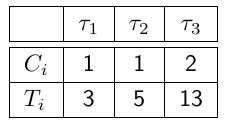
\includegraphics[width=0.25\textwidth]{./figures/1_tasks.png}
    \begin{itemize}
      \item what can be the maximum value of $U_s$ such that the whole set (i.e. periodic tasks and the \alert{TBS}) is schedulable with \alert{EDF}?
    \end{itemize}
  \end{tasknoinc}
  \begin{requirementsnoinc}
    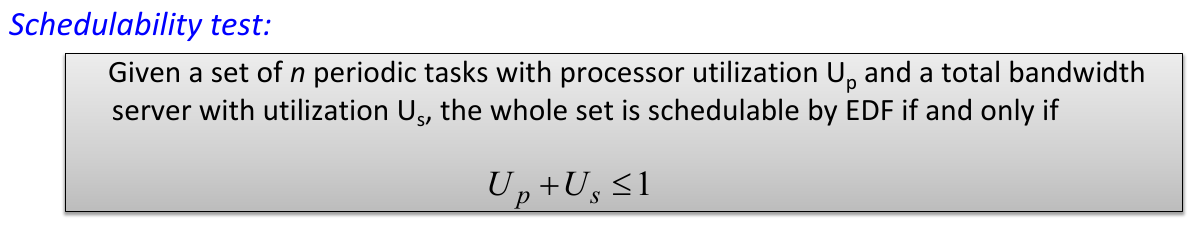
\includegraphics[width=\textwidth]{./figures/schedulability_test.png}
    \begin{itemize}
      \item \alert{processor utilization factor:} $\displaystyle U=\sum_{i=1}^n \frac{C_i}{T_i}$
    \end{itemize}
  \end{requirementsnoinc}
  \begin{solution}
    \begin{itemize}
      \item \alert{Maximum utilization of the Total Bandwidth Server:} $U_{s, \max }=1-U_p=1-(\frac{1}{3}+\frac{1}{5}+\frac{2}{13})=\frac{61}{195} \approx 0.3128$
    \end{itemize}
  \end{solution}
\end{frame}

\begin{frame}[allowframebreaks]{}{}
  \begin{solution}
    \begin{itemize}
      \item First, we need to order the tasks by increasing release time $r_i: J_4, J_6, J_5$. Then, we calculate the deadlines with $d_i=\max \left(r_i, d_{k-1}\right)+\frac{C_k}{U_s}$, where $d_{k-1}$ denotes the previously calculated deadline $(k-1$ means the predecessor in the ordering according to the release time):
  \begin{itemize}
    \item $d_4=\max \left(r_4, d_0\right)+2 / 0.25=0+8=8$
    \item $d_6=\max \left(r_6, d_4\right)+1 / 0.25=10+4=14$
    \item $d_5=\max \left(r_5, d_6\right)+1 / 0.25=15+4=19$
  \end{itemize}
    \end{itemize}
  \end{solution}
  \begin{solution}
    \centering
    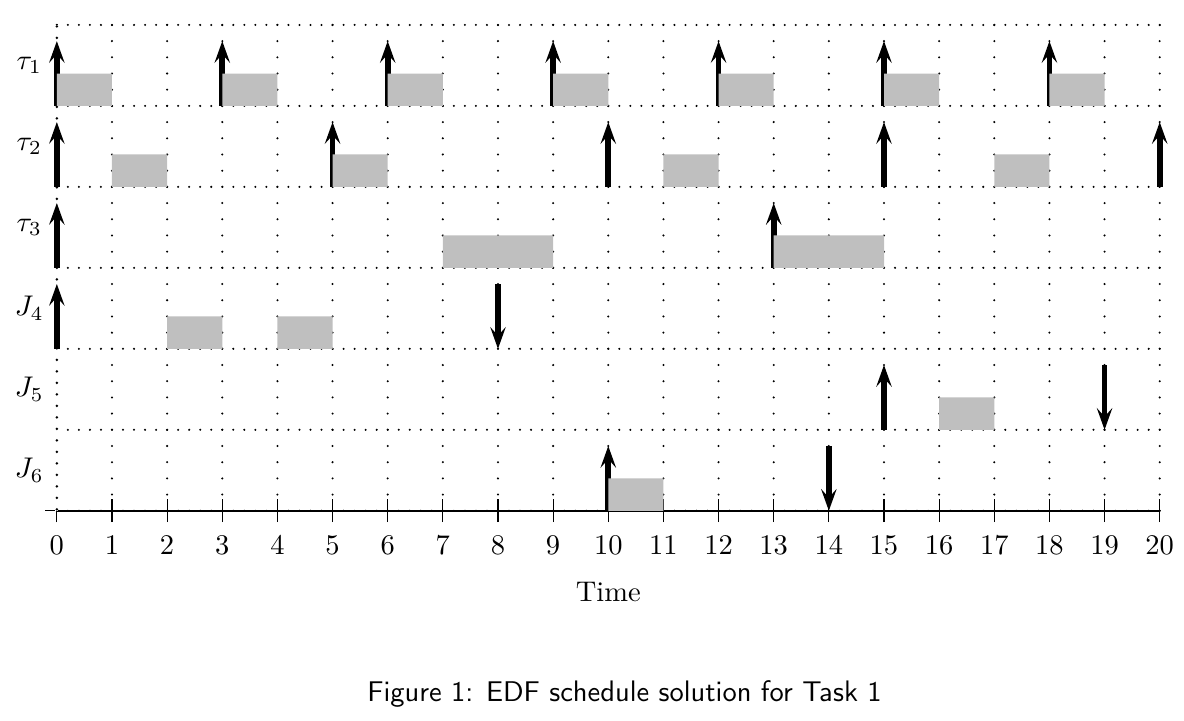
\includegraphics[height=0.6\paperheight]{./figures/1_sol.png}
  \end{solution}
\end{frame}
